\documentclass[12pt]{article}

\usepackage[utf8]{inputenc}
\usepackage[T1]{fontenc}
\usepackage[margin=2.4cm]{geometry}
\usepackage{xcolor}
\usepackage[skins,breakable]{tcolorbox}
\usepackage{enumitem}
\usepackage{titlesec}
\usepackage{hyperref}
\usepackage{tikz}
\usetikzlibrary{arrows.meta,positioning}
\usepackage{fontspec}
\setmainfont{TeX Gyre Pagella}

% ---------------------------------------------------------------
% Same palette as the slide deck and script, for visual continuity
% ---------------------------------------------------------------
\definecolor{sovDark}{RGB}{18,32,51}
\definecolor{sovDarkAlt}{RGB}{27,46,74}
\definecolor{sovGold}{RGB}{214,164,64}
\definecolor{sovRed}{RGB}{163,44,58}
\definecolor{sovGrey}{RGB}{92,102,117}
\definecolor{sovPaper}{RGB}{250,248,244}
\definecolor{sovGreen}{RGB}{58,110,89}

\hypersetup{
  colorlinks=true,linkcolor=sovDark,urlcolor=sovDark,citecolor=sovDark,
  pdftitle={Digital Sovereignty for Kashmir},
  pdfauthor={Owais Saleem},
  bookmarksopen=true
}

\titleformat{\section}{\normalfont\Large\bfseries\color{sovDark}}{\thesection}{0.6em}{}
\titlespacing*{\section}{0pt}{16pt}{6pt}
\titleformat{\subsection}[block]{\normalfont\large\bfseries\color{sovDarkAlt}}{}{0em}{}
\titlespacing*{\subsection}{0pt}{10pt}{4pt}

% Soft, airy highlight for visionary quotes
\newtcolorbox{vision}{
	enhanced, breakable,
	colback=sovGold!12,          % 12% Gold, 88% White -> very soft warm glow
	colframe=sovGold!40,         % 40% Gold for a muted, elegant border
	coltext=sovDark,             % Dark navy for maximum readability
	boxrule=0.8pt, arc=3pt,
	left=10pt, right=10pt, top=8pt, bottom=8pt,
	fontupper=\itshape
}


\pagecolor{sovPaper}
\color{sovDark}

\setlength{\parskip}{5pt}
\setlength{\parindent}{0pt}

\begin{document}

% ================================================================
\begin{center}
  {\LARGE\bfseries\color{sovDark} Digital Sovereignty - a modest proposal}\\[6pt]
  {\Large\color{sovGrey} A Vision, and a Path We Have Already Started Walking}\\[10pt]
  {\normalsize Owais Saleem \hspace{4pt}\textbar\hspace{4pt} July 2026}
\end{center}

\vspace{6pt}
{\color{sovGold}\rule{\linewidth}{1pt}}
\vspace{6pt}

Every day, someone even in a remote region like Kashmir borrows a library book through an app, a farmer
cooperative logs a harvest, a student's record is updated at school. Each of these
small acts of digital life is quietly stored on a server none of us own, reachable
under a law none of us wrote. This note lays out what a different path
looks like, and why the coming few years are the right window to start building it.

\section{The uncomfortable fact we live with every day}

Roughly two-thirds of the world's cloud computing spend is concentrated in three
American companies.\footnote{Indicative figures based on public analyst estimates
(Synergy Research Group, Canalys, 2025--26 market share reporting).} Nearly every
app, portal, or database a small organisation in Kashmir builds today ends up
running, physically and legally, on one of their machines --- regardless of which
country the data center itself sits in. Since 2018, US law has required any
American company to hand over data on government request, no matter where in the
world the server holding it is located. A platform advertising ``data residency in
India'' on top of American infrastructure is offering a comforting label, not
sovereignty.

Can a small group of ambitious youth and talented students make a difference? Can we contribute to laying the foundation of something that will enable people to dream of disentangling themselves from the chains of Western corporate digital supremacy? The answer is an unflinching yes—but only if we stop waiting for the perfect and convenient solution and start building.

\begin{vision}
The question was never whether we depend on digital infrastructure --- we already
do, every day, for things that matter. The real question is: whose infrastructure,
under whose law, and who profits from it.
\end{vision}

\section{What sovereignty actually means here}

This is not an argument for disconnecting, nor for reinventing technology that already works well. It is an argument about ownership of a small number of foundational layers—where things are hosted, who hands over our data and to whom, and what happens to a community's data if a distant vendor changes its terms or raises its price.

The vision is a shared, open technical foundation—the basic plumbing that almost any digital service needs: a place to store data safely, a way to verify who a user is, a way to keep files, and a way to keep the lights on when the grid or the network falters. Built once, built openly, and hosted on infrastructure that this region actually owns \& controls. Any local institution that needs a digital presence—a library, a farmer cooperative, a clinic keeping patient records, a school archiving its own history, or even our moments, stories, pictures \& videos—should be able to build on that foundation, rather than each independently renting the same dependency from the same distant companies.

Two design choices make this realistic rather than idealistic. First, every layer of this foundation will be built from open, freely licensed software, so no single vendor—foreign or local—can hold it hostage. Second, it is designed to be regional rather than purely local: resilient when any one city or building loses power or connectivity, yet never dependent on foreign jurisdiction.



\section{Proof before promise: what is already being built}

This vision is not starting from a blank page, and it should not be mistaken for
a purely hypothetical ask. Small, independent projects are already live and
already serving real people in the region. The latest \emph{Marsiya} App, built by the
Dreamer's Institute, is one such example. A community library portal is another,
already handling real book donations, loans, and requests for real users. Neither
was built as a grand infrastructure statement --- each simply set out to solve one
concrete, local problem, and did.

\begin{vision}
	What these early projects have in common matters more than any one of them individually: each was built by a small local team with limited resources, and each currently rents its underlying infrastructure from the very same distant platforms this note describes as the long-term problem. They are proof that the demand is real and the technical skill to build for it already exists here. What they do not yet have is a shared, regionally owned home to run on. OLK's current technical stack and database structure are open source from top to bottom—and ready to be hosted on a local server.\footnotemark
\end{vision}
\footnotetext{To be discussed in detail in our upcoming meeting.}
That is the opportunity in front of us: not to start a first project, but to give
the projects that already exist --- and the ones that have not been imagined yet
--- a foundation that belongs to this region, so that scaling one of them up, or
starting the next one, is no longer a decision that has to be made one distant
subscription at a time.

\section{The path: three stages, not one leap}

Owning meaningful infrastructure sounds like it requires a large facility and a
large budget on day one. It does not. The realistic path is staged, and each
stage is deliberately sized to the confidence and resources available at that
point.

\begin{center}
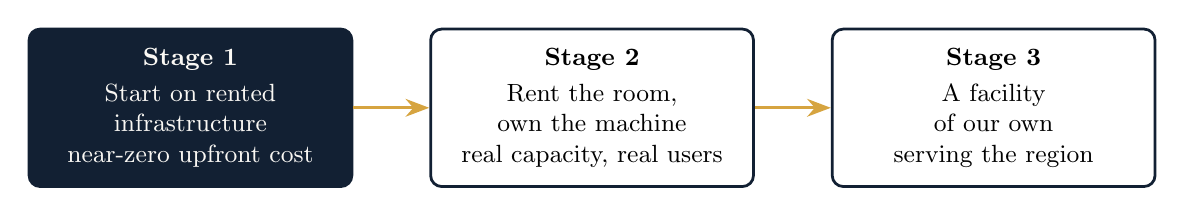
\begin{tikzpicture}[
    stage/.style={rounded corners,draw=sovDark,line width=1pt,fill=white,
      minimum width=4.1cm,minimum height=2cm,align=center,font=\small,inner sep=6pt},
    hl/.style={fill=sovDark,text=sovPaper},
    arr/.style={-{Stealth[length=3mm]},line width=1.2pt,draw=sovGold}
  ]
  \node[stage,hl] (s1) at (0,0)    {\textbf{Stage 1}\\[2pt]Start on rented\\infrastructure\\near-zero upfront cost};
  \node[stage]     (s2) at (5.1,0) {\textbf{Stage 2}\\[2pt]Rent the room,\\own the machine\\real capacity, real users};
  \node[stage]     (s3) at (10.2,0){\textbf{Stage 3}\\[2pt]A facility\\of our own\\serving the region};
  \draw[arr] (s1) -- (s2);
  \draw[arr] (s2) -- (s3);
\end{tikzpicture}
\end{center}

In the first stage, services run on infrastructure rented cheaply from outside
the region, at near-zero upfront cost, while the team behind them builds the
operational skills --- running servers, keeping backups, monitoring uptime ---
that every later stage depends on. In the second stage, the team moves to
renting physical space, power, and connectivity inside an existing facility,
while the server hardware itself belongs to us. This is where a real pilot
lands: capable of serving tens of thousands of users, not a demonstration. In
the third stage, the region has its own dedicated facility, with redundant power
and connectivity, serving as shared infrastructure for many local institutions
at once.

The point of staging it this way is that nothing gets thrown away as we advance.
Every stage runs the same open software, on the same foundation, for the same
projects. Moving from one stage to the next is an upgrade, not a rebuild --- which
means a modest first step is not a compromise on the vision, it is the fastest
honest route toward it.

\section{Why now}

Three trends are converging in a way that makes this the right moment, not an early one.

\textbf{The physical foundation is catching up.} Reliability of the regional power grid has been improving; efficient UPS systems are becoming affordable; and integrating renewable sources has not only become realistic but is also highly encouraged by existing policies—closing a gap that would have made this proposal premature not long ago.

\textbf{The software layer has matured.} The open-source tools needed to run this kind of shared infrastructure—databases, authentication, storage, hosting—are now mature, well documented, and designed to be self-hosted from day one. Building on them today is a matter of deployment and operations, not unproven research.

\textbf{The community already exists.} As the previous section showed, the builders, the demand, and the early proof points are not hypothetical—they are already here, scattered across a handful of small independent projects. What is missing is not talent or appetite. It is a shared foundation, and the modest resources needed to start building it deliberately rather than accidentally.

\begin{vision}
	We are not choosing between staying dependent and building a data center overnight. We are choosing the order in which we build confidence, skill, and capability—starting now, with what we already have.
\end{vision}

\section{An invitation}

This note is deliberately brief, and deliberately light on the engineering detail behind it. That detail exists, has been worked through to a large extent, and will be presented—with a concrete first-stage plan, a realistic budget, and a clear list of the roles and skills still needed—at the presentation this note is meant to introduce.

If the argument above resonates—that each region should own the infrastructure its community life increasingly depends on; that the pieces to start doing so are closer at hand than they might seem; and, most importantly, that it can be efficiently built by our youth and students—then the invitation is simple: come, be part of the plan, and help decide what gets built next.

\vspace{8pt}
\begin{center}
	{\large\color{sovDark} Our data. Our servers. Our region.}\quad
	{\large\color{sovGold}\textbf{Let's begin.}}
\end{center}

\end{document}
